\documentclass[12pt]{article}
\usepackage{fullpage}
\usepackage[margin=1in]{geometry}
\usepackage[stable]{footmisc}
\usepackage{graphicx}
\usepackage{amssymb}
\usepackage{IEEEtrantools}
\usepackage{lineno}
\usepackage{amsmath}
\usepackage{epstopdf}
\usepackage{parskip}
\usepackage{authblk}
\usepackage[authoryear]{natbib}
%\setlength{\parskip}{20pt}
\linespread{1.6}
\date{}

\DeclareGraphicsRule{.tif}{png}{.png}{`convert #1 `dirname #1`/`basename #1 .tif`.png}


%%	math short-cuts
\def \ve{\varepsilon}	% epsilon used for metabolic rate
\def \la{\lambda}	% lambda
\newcommand{\eref}[1]{( {#1})}

%%	new commands for referencing figures and tables and sections
\newcommand{\fref}[1]{Figure~\ref{#1}}	% inline figure ref
\newcommand{\fpref}[1]{Fig.~\ref{#1}}	% parenthetical figure ref
\newcommand{\tref}[1]{Table~\ref{#1}}	% table ref
\newcommand{\sref}[1]{Section~\ref{#1}}	% table ref
%\linenumbers

\title{\Large \textbf{Generating oscillations in MERA: differentiate generation time from allocation period}}

\author{Jade, Nov 16}

\begin{document}
\maketitle
\raggedright
\large
\setlength{\parindent}{15pt}

From results in the previous write-ups we can see that, under the current framework of MERA, for both the single species case and the multiple competitors case, population size does not oscillate even when the (discrete) intrinsic growth rate $r$ is very high (as opposed to the predictions of the logistic growth equation). Through time, each species converges gradually to its steady state and stays there permanently once it is reached. 

In this write-up I will first examine the temporal assumptions of MERA compared to the discrete and continuous logistic growth equations to infer which part of our assumptions might eliminate oscillations. Next I will prove that the relaxing of these assumptions does generate oscillations under the MERA framework. The conclusion is that the difference between generation time (see definition below) and allocation period is at the root of population oscillations in MERA predictions.

\section{A projection: oscillation and time lag}

We all know that the discrete logistic growth equation leads to oscillations around the steady state when the intrinsic growth rate is high, while its continuous counterpart does not. Although there could be a number of explanations to this, my point of view is that, in the discrete logistic growth model, there is a time lag (the length of the time interval $\Delta t$) for the population growth rate to react to the density dependence effects imposed by its own abundance. A more elaborate way to say it is that during this time interval, population size and the form of density dependence is not updated and the population grows at the same rate based on information at the beginning of the interval, creating a chance for over shooting. In the continuous model, however, there is no time lag and therefore population growth rate is instantly updated, leaving no chance for over shooting. 

Now let's look at MERA. In MERA, the density dependence of population growth is realized through the resource allocation process. So far we have assumed that the population size is updated every time (and only when) resource is allocated. This means that there is no time lag for the population to react to the density dependence effects imposed by its abundance. Therefore, although MERA is seemingly a discrete model (since resource allocation happens in discrete time steps), from the argument above we can see that it is actually more like a model for continuous growth, which is probably the reason why we do not see oscillations in MERA predictions. 

So far it is merely an educated guess. But it is easy to test: if we introduce time lag into MERA so that population size does not change every time resource is allocated, in other words resource needs to be accumulated for multiple allocation periods before population size can be updated, different population dynamics (possibly with oscillations) is expected. 

In population growth models, the length of $\Delta t$ is usually interpreted as generation time, which by the most generally accepted definition in demography and population biology is the average time between two consecutive generations in the lineages of a population. Here I am going to use this term to represent the length of waiting time (during which resource can be allocated multiple times and accumulated) between two consecutive changes in population size. You can see the connections between these two definitions but still there are distinctions. I will discuss about this later.

\section{Introducing species specific generation time into MERA}

To relax the previous MERA assumption of population generation time being the same with resource allocation period, here an extra parameter $d t_{G,i}$ is introduced to represent the population generation time for species $i$. When $d t_A$ is used to annotate the length of resource allocation period, the ratio $d t_{G,i}/d t_A$ is the number of times resource from allocation has to be accumulated before the change in population size takes place. Practically, we will use the largest previous integer of this ratio, assuming that the resource can only be allocated at the end of an allocation period.

The previous single species model is equivalent to $d t_{G,i}=d t_A$, or growth is only accumulated for one allocation period before added on to the population. This leads no oscillations under all conditions (Fig.1).

\begin{figure}
 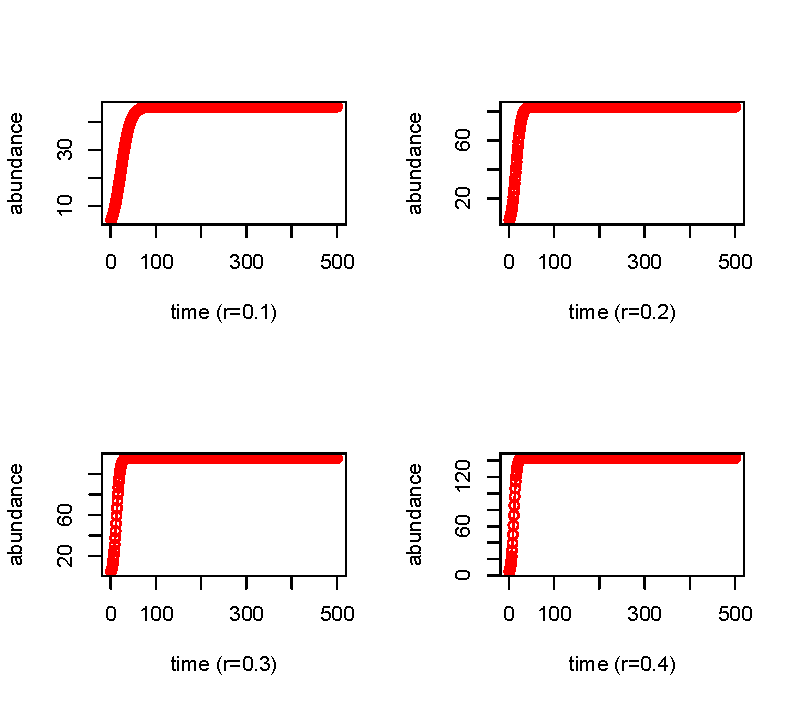
\includegraphics[width=\textwidth]{1sp_no_sojourn.pdf}
 \caption{Single species growth with no time lag ($d t_{G,i}=d t_A$)}
For all four graphs $ N_{1,t=0}=5, \theta_1=1, D_{r,1} = 0, R_0=500$. The value of $r_{discrete}$ is shown under the x-axis.
\end{figure}

Further refine the time intervals (keeping steady state and intrinsic growth rate constant). See if dynamics change. (The shape might not change at all!!)

As will be proved later, when $d t_{G,i}=d t_A \to 0$, the resulting growth function is exactly the same as the continuous-time logistic growth function

\subsection{Single species case: increased oscillations with $D_r$ and discrete intrinsic growth rate $r_{discrete}$}

Now let's look at the case where $G_1=10$, so that generation time is ten times as long as one allocation period, or growth (positive or negative) has to be accumulated for 10 allocation periods before added on to the population (Fig. 2 \& 3).

\begin{figure}
 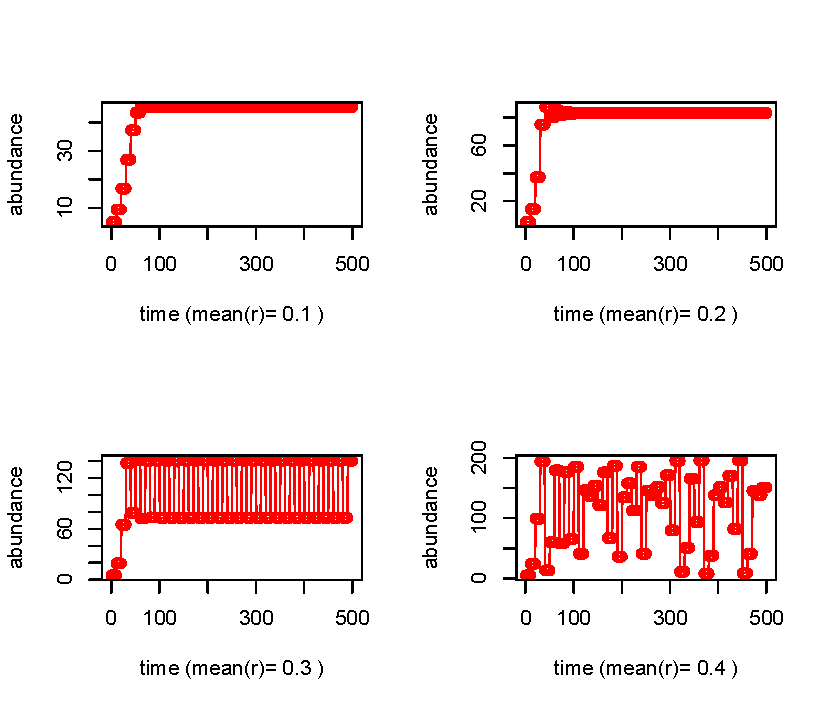
\includegraphics[width=\textwidth]{1sp_sojourn.pdf}
 \caption{Single species growth with time lag ($G_1=10$)}
For all four graphs $ N_{1,t=0}=5, \theta_1=1, D_{r,1} = 0, R_0=500$. The value of $r$ is shown under the x-axis.
\end{figure}

\begin{figure}
 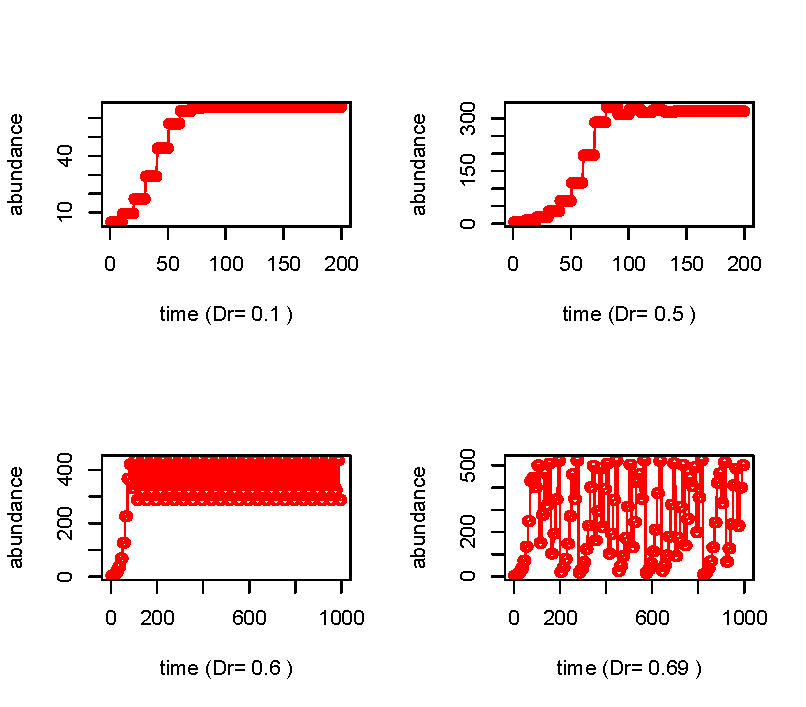
\includegraphics[width=\textwidth]{1sp_sojourn_Dreffect.pdf}
 \caption{$D_r$ effect on single species growth with time lag ($G_1=10$)}
For all four graphs $ N_{1,t=0}=5, \theta_1=1, r_1= 0.1, R_0=500$. The value of $D_{r,1}$ is shown under the x-axis.
\end{figure}

Comparing Fig. 1 and Fig. 2 we can see that, although it does change oscillation patterns, increasing species generation time (with everything else unchanged) does not seem to change the mean value of steady state abundance. 

From Fig. 2 and Fig. 3 we can see that, when the species generation time is not the same as the resource allocation period, all else equal, the bigger the $r$ or the bigger the $D_r$, the more oscillations in population dynamics. Actually when you look across the graphs in each figure, you'll see that the effect of increasing $r$ and $D_r$ is very similar to that of the intrinsic growth rate in the logistic growth function. 


\section{Discussion}

\subsection{Tradeoff for $r$ and $D_r$: high mean vs high oscillation}
In the previous write-up (Nov 12) I have proved that the steady state abundance of a single species community is determined by the following equation
  \begin{equation}
\hat{N_1} =[ \frac{1}{r_1 (\frac{R_0}{\theta_1}- \hat{N_1})}]^{\frac{1}{D_{r,1}-1}}
  \end{equation}
Eq. 1 is simply Eq. 13 in write-up Nov 12 for the single species case. It shows that the steady state abundance of the single species case is solely determined by three parameter values: $r_1$, $D_{r,1}$ and the ratio $\frac{R_0}{\theta_1}$. From the results in this write-up (increasing generation time does not affect the steady state abundance), we have shown that Eq. 1 holds even when generation time is not the same as allocation period. This means that higher $r$ will always lead to higher mean steady state abundance, regardless of the magnitude of generation time. However, when generation time is much higher than allocation period,  higher $r$ leads to more drastic oscillations, reducing the stability of the population. Similarly for $D_r$, although high $D_r$ leads to high mean steady state abundance, it also generates more oscillations, increasing the risk of extinction over time.

These results provide a parsimonious explanation to why not all species take an $r$ strategy or high $D_r$ without extra assumptions on fitness or density dependence of death and competition (although reasonable connections with these mechanisms might be potentially established).

\subsection{Allocation period as one extra parameter in growth functions}

From Eq.1, if we further assume that for this single species $D_{r,1}=0$ (see discussion in Nov 12 write-up), the above can be simplified into 
   \begin{equation}
\hat{N} = \frac{r}{r+1}\frac{ R_0}{\theta} 
  \end{equation}

Notice that the $r$ here is not the growth rate over a generation time, but the maximal growth rate of the species over a resource allocation period. The relationship between this $r$ and the rate over a generation time $r_{logi}$ as appears in the discrete logistic function is

\begin{equation}
 \frac{ \mbox{log} (1+r) }{A} = I_r = \frac{ \mbox{log} (1+r_{logi}) }{G}
\end{equation}

Where $A$ is the length of the allocation period. Eq. 3 is obtained by assuming that the two discrete growth rates correspond to the same instantaneous intrinsic growth rate $I_r$. 

In the discrete logistic growth function, the shape of population dynamics given the initial abundance is determined once the values of steady state abundance $\hat{N}$, the discrete intrinsic growth rate $r_{logi}$ and the generation time $G$ are determined. Here from Eqs. 2 and 3 we can see that, even if $r_{logi}$, $\hat{N}$ and $G$ are determined, the values of $r$, $A$ and $R_0/\theta$ are not pinned down unless at least one of them is known. This means that for any given logistic growth function parameter setting, there can be multiple corresponding MERA parameter settings. This extra degree of freedom is due to the newly introduced flexibility in the relationship between the two time periods: the resource allocation period $A$ and the species generation time $G$. Fig. 5 shows when $r_{logi}$, $\hat{N}$ and $G$ are controlled, how different allocation period $A$ leads to different population dynamic patterns:


When $A$ gets smaller, there are more oscillations, especially when $r_{logi}$ is high. 

$A$ is an independent parameter. When close to 0 it might generate dynamics very close to the logistic growth function. Especially when $r_{logi}$ gets higher, $A$ plays a more and more important role in determining the oscillation pattern.

Derive the approximation of growth function when $A$ approaches 0. In the following I will use $dt$ in place of $A$. $I_r$, $I_R$ and $I_\theta$ are instant values.

\begin{equation}
(N + dN)^2 = (I_r dt N  - dN) [\frac{I_R}{I_\theta} - (N+dN)]
\end{equation}

To control for steady state abundance, set $dN=0$ for Eq. 4 we can solve the steady state abundance: 
\begin{equation}
\hat{N} = \frac{I_R}{I_\theta} \frac{I_r dt+1}{I_r dt} 
\end{equation}

Substitute this into Eq. 4 we have
\begin{equation}
(N + dN)^2 = (rN dt - dN) [\hat{N} \frac{I_r dt+1}{I_r dt} - (N+dN)]
\end{equation}

Expand the expression and get rid of the small terms (those with dN and/or dt) we can get

\begin{equation}
\frac{dN}{dt}_{dt = \lim{A \to 0}} = \frac{I_rN (\hat{N}-N)}{\hat{N}}
\end{equation}

Exactly the same as the continuous logistic growth function. Now we see that continuous limit matches, have the reason to believe that discrete logistic growth function assumes continuous resource allocation with larger generation times.

Find dt that will prove this point. (For a reasonable $r$ value, smaller $dt$ generates dynamics that more and more resemble the logistic growth function).

Reveal that continuous resource allocation is not necessarily the case for all systems. The longer the resource allocation period, all else equal, increases steady state abundance (and coexistence?) and stability.

$D_r$ might still play into the continuous solution. Try to solve one with general $D_r$.

Or $D_r=1$. $I_R/I_\theta r = \hat{N} + 1/r$



\subsection{How to test}
If there are species with high $r$, high $G$ but apparently more stability, this suggests discrete resource allocation. 

Predict that annual or bump systems have more stability.

Important for predator-prey interactions with differential generation time.

Since generation time is species specific, this is a particularly important assumption to explore for both the single species case and multiple species cases where generation time not only differs from allocation period, but also potentially varies among species.


\section{Appendix: Multiple competitors case: differential generation time among species}
\begin{figure}
 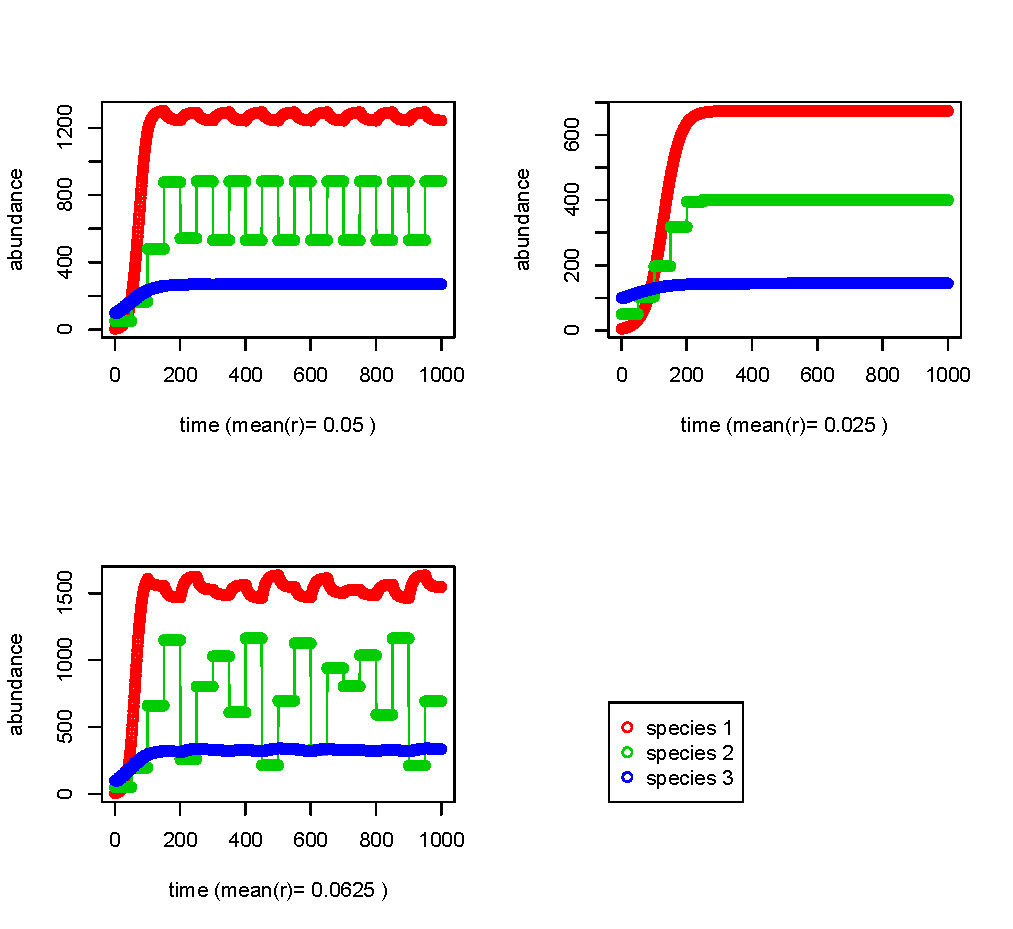
\includegraphics[width=\textwidth]{oscillation_r_effect.pdf}
 \caption{Multiple species competing for one fundamental resource with differential generation time ($G_1=1, G_2=50, G_3=10$)}
For all four graphs $ N_{1,t=0}=5, N_{2,t=0}=50,N_{3,t=0}=100, D_{r,1}=D_{r,2}=D_{r,3}=0.1, \theta_1=\theta_2=\theta_3=1, r_1: r_2:r_3= 8:5:2, R_0=10000$. The mean value of $r$s is shown under the x-axis.
\end{figure}

\begin{figure}
 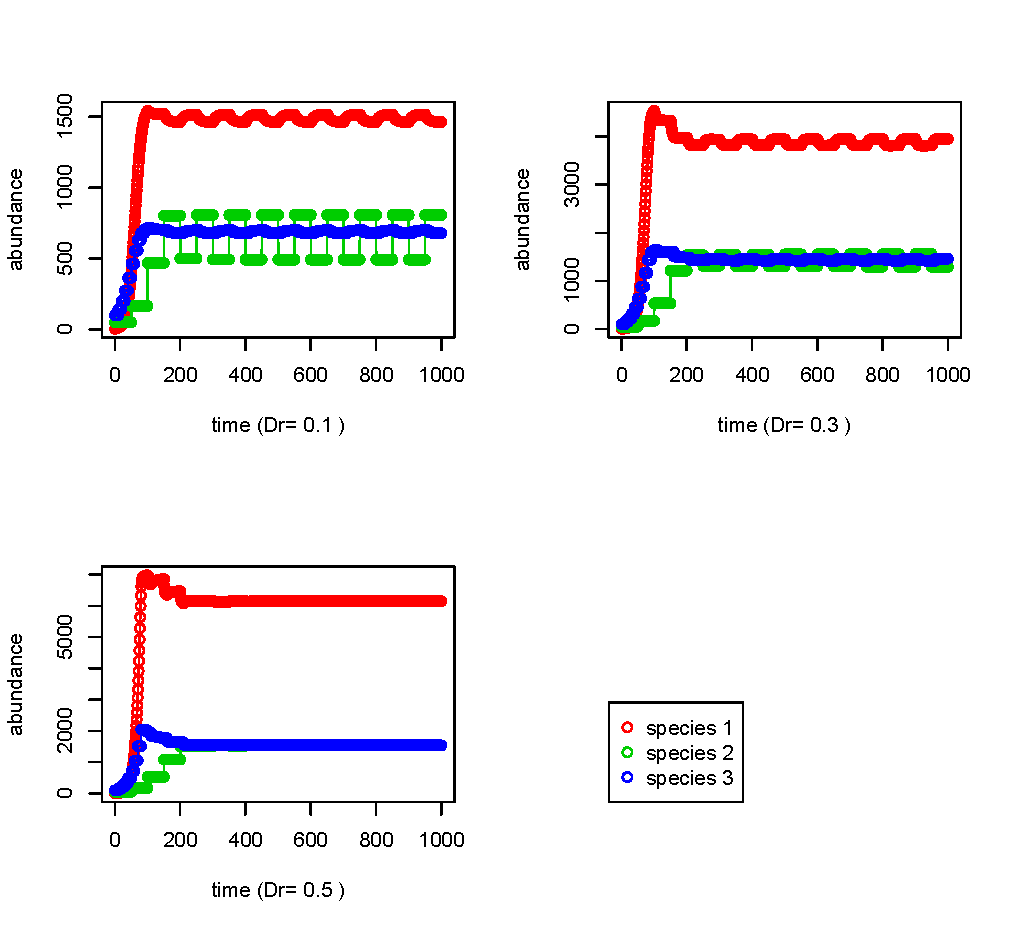
\includegraphics[width=\textwidth]{oscillation_Dreffect.pdf}
 \caption{$D_r$ effect on multiple species competing for one fundamental resource with differential generation time ($G_1=1, G_2=50, G_3=10$)}
For all four graphs $ N_{1,t=0}=5, N_{2,t=0}=50,N_{3,t=0}=100, \theta_1=\theta_2=\theta_3=1, r_1=0.08, r_2 =0.05, r_3= 0.02, R_0=10000$. $D_r$ is set to be the same for all species, the value is shown under the x-axis.
\end{figure}

From Fig. 4 and Fig. 5 we can see that, when there are species with generation time bigger than 1, populations for all species (including those with generation time equal to 1) oscillate. Fig. 4 shows that similar to the single species case, bigger $r$ for all species leads to more oscillations. However, Fig. 5 shows that bigger $D_r$ for all species leads to reduced oscillations, which is contrary to the single species case. This suggests that there is probably a tradeoff between intra- and interspecific competition in generating oscillations. In future analysis I will look into more parameter settings.





\end{document}